\section{Evaluation}

The last chapter presented an implementation of the method to infer time, size and cost bounds.
This chapter evaluates this implementation against other methods.

For this purpose, two different approaches are used.
First, some selected examples are presented that show the benefit of the presented method in contrast to the method of \cite{koat}.
Second, the implementation is evaluated on an example set of programs.
This set of programs is defined and used by comparable tools with the same objective of inferring time bounds for integer programs.

\subsection{Evaluating Selected Examples}

This section presents two selected examples to compare the results of the new method with the results of the method of \cite{koat}.
This selection is chosen to show the benefits of the new method and is by no means representative.
Nevertheless, it is able to show the potentials of the new method.

The first evaluated example is the motivational program from the introduction in Figure \ref{fig:motivational_example}.

\begin{figure}
  \centering
  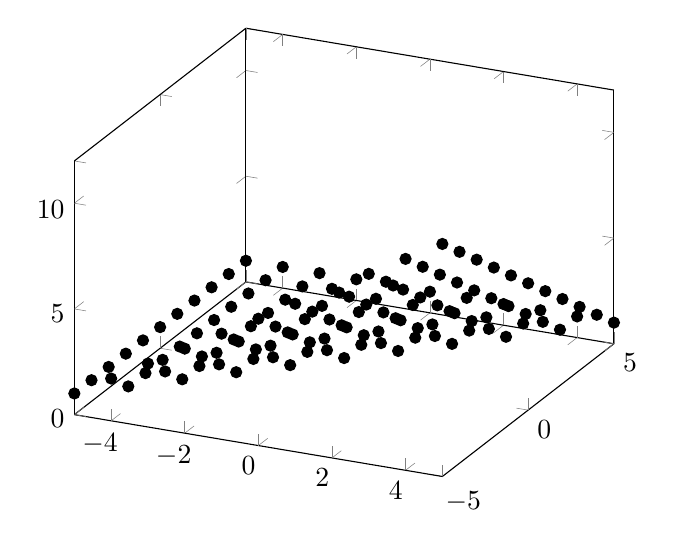
\begin{tikzpicture}
    \begin{axis}
      \addplot3 [
        unbounded coords=jump,
        mesh,
        shader=interp,
        samples at={-5,...,5},
        samples y={11},
        only marks,
      ] {1+max(x-y,0)};
    \end{axis}
  \end{tikzpicture}
  \hfil
  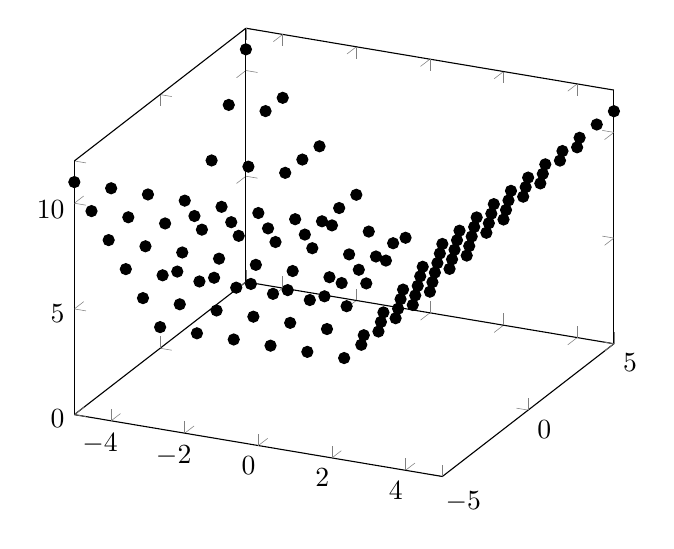
\begin{tikzpicture}
    \begin{axis}
      \addplot3 [
        unbounded coords=jump,
        mesh,
        shader=interp,
        samples at={-5,...,5},
        samples y={11},
        only marks,
      ] {1+abs(max(x,-y))+abs(max(x,-y))};
    \end{axis}
  \end{tikzpicture}
  \caption{Evaluation of the motivational example}
  \label{fig:motivational_evaluation}
\end{figure}


For this program, the new method derives a time complexity of $\maxO{x-y}$, while KoAT \cite{koat} infers a time complexity of $\abs{x}+\abs{y}$.
In the new method, we assume that we have two input states $\lstate$ and $\ustate$.
KoAT \cite{koat} is defined with a single input state $m$ such that $m(v) = \maximum{-\lstate(v),\ustate(v)}$ for each variable $v \in \PVSet$.

Figure \ref{fig:motivational_example} provides two three-dimensional graphs.
The left graph plots the time complexity $\maxO{x-y}$ of the new method and the right graph plots the time complexity $\abs{x}+\abs{y}$ of KoAT \cite{koat}.
We consider input states $\lstate$ and $\ustate$ with $\lstate(v) = \lstate(v')$ and $\ustate(v) = \ustate(v')$ for all variables $v, v' \in \PVSet$.
The graphs show that the time complexities are the same if $-\lstate = \ustate$.
This is the expected result, as $-\lstate = \ustate$ implies that $m = -\lstate = \ustate$.
The new method infers a lower time complexity if the value of $-\lstate$ and $\ustate$ diverges.
The biggest gain is achieved, when $\lstate = \ustate$.
That is if an exact state $\lstate = \valuation = \ustate$ is given.

The second evaluated example is the program presented in the cost bound chapter \ref{fig:cost_ranking_function}.

\begin{figure}
\centering

\begin{tikzpicture}[->,>=stealth',auto,node distance=5cm,
    thick,
    main node/.style={circle,draw,font=\sffamily\Large\bfseries},
    aligned edge/.style={align=left}]

  \node[main node] (0) {$\location_0$};
  \node[main node] (1) [right of=0] {$\location_1$};

  \path[every node/.style={font=\sffamily\small}]
    (0) edge[aligned edge] node[above=0.2cm] {$t_0$} node[below=0.2cm] {$\update = \emph{id}$} (1)
    (1) edge[aligned edge, loop above] node[left=0.2cm] {$t_1$} node[below right=0cm and 0.5cm] {$\update(x) = x - y$\\$\update(y) = y$\\$\guard = \braced{y > 0, x > y}$\\$\cost(t_1)=y$} (1)
    ;
\end{tikzpicture}

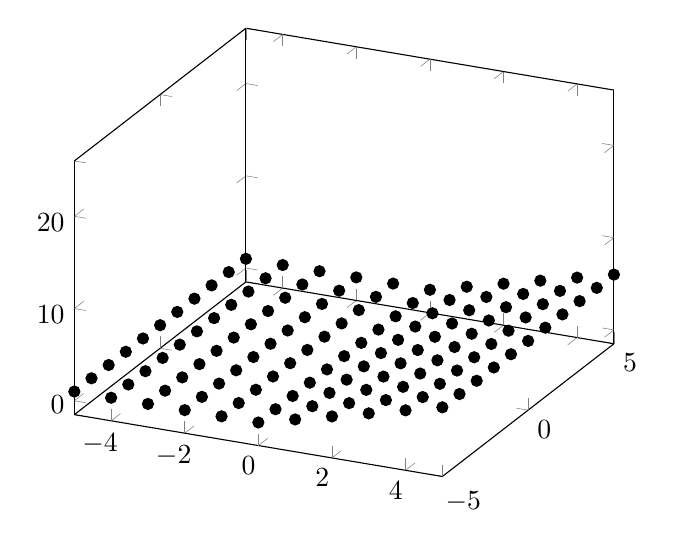
\begin{tikzpicture}
  \begin{axis}[zmax=26]
    \addplot3 [
      unbounded coords=jump,
      mesh,
      shader=interp,
      samples at={-5,...,5},
      samples y={11},
      only marks,
    ] {1+max(x,0)};
  \end{axis}
\end{tikzpicture}
\hfil
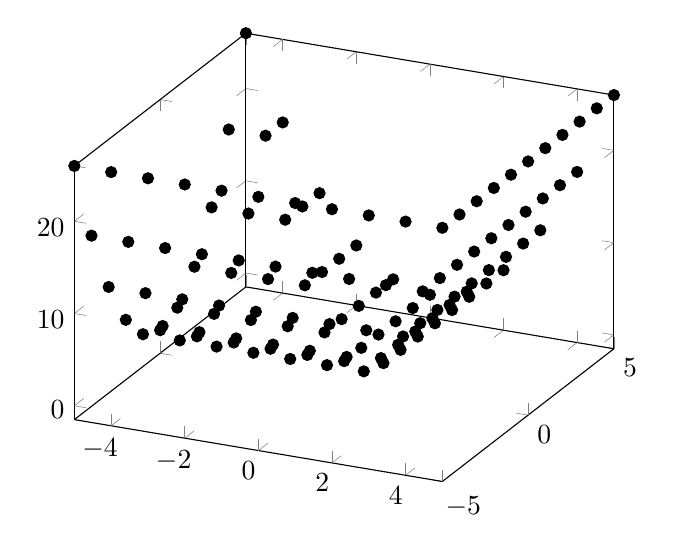
\begin{tikzpicture}
  \begin{axis}[zmax=26]
    \addplot3 [
      unbounded coords=jump,
      mesh,
      shader=interp,
      samples at={-5,...,5},
      samples y={11},
      only marks,
    ] {1+abs(max(x,-y))*abs(max(x,-y))};
  \end{axis}
\end{tikzpicture}

\caption{Evaluation of an example with cost ranking functions yielding a benefit}
\label{fig:cost_ranking_function}
\end{figure}


As already mentioned, the presented method is able to compute a cost bound $\UCost(t_1) = \maxO{x}$ for the transition $t_1$.
Therefore $1 + \maxO{x}$ is a cost bound for the whole program.
Since \cite{koat} does not consider cost ranking functions, its method is only able to compute a cost bound $1 + \abs{x} \cdot \abs{y}$ for the whole program.

The functions are plotted with the same assumptions as the previous example.
The left graph plots the cost complexity $1 + \maxO{x}$ of the new method and the right graph plots the cost complexity $1 + \abs{x} \cdot \abs{y}$ of the method of \cite{koat}.
In this example, the new method yields better results for all input states $\lstate = \ustate$.

\subsection{Evaluating an Example Set}

This section evaluates the presented implementation on an example set.
This set is a collection of 689 examples introduced by other tools.
We compare the presented method to the results presented in \cite{koat}.
These results include the results of the tool KoAT itself as well as the results of the tools CoFloCo \cite{cofloco1, cofloco2}, Loopus \cite{loopus1, loopus2}, KoAT-TACAS \cite{leike2014ranking}, PUBS \cite{pubs1, pubs2} and Rank \cite{rank}.

For the comparison of the results, it is necessary to project the resulting bounds in $\BoundSet(\PVSet)$ to their asymptotic complexity class.
The following definition introduces a projection, such that for every bound $b \in \BoundSet(\PVSet)$ the resulting asymptotic complexity $\complexity(b)$ is a valid overapproximation of the actual complexity.

\begin{definition}[Approximation of the Asymptotic Complexity]
  Let $\VSet$ be a finite set of variables.
  Let $\BoundSet(\VSet)$ be the set of bounds over the variables $\VSet$.
  Let $\landau$ be the landau symbol for asymptotic complexity.
  Then, $\complexity$ is a function which assigns each bound an overapproximation of its asymptotic complexity.
  \begin{align*}
    \complexity(\infty) &= \landau(\infty) \text{ for } \infty \in \BoundSet(\VSet) \\
    \complexity(k) &= \landau(1) \text{ for all } k \in \mathbb{N} \subseteq \BoundSet(\VSet) \\
    \complexity(v) &= \landau(n) \text{ for all } v \in \VSet \subseteq \BoundSet(\VSet) \\
    \complexity(-b) &= \complexity(b) \text{ for all } b \in \BoundSet(\VSet) \\
    \complexity(b_1 + b_2) &= \landau(f_1 + f_2) \text{ for all } b_1, b_2 \in \BoundSet(\VSet) \\
    & \text{ with } \complexity(b_1)=\landau(f_1) \text{ and } \complexity(b_2)=\landau(f_2) \\
    \complexity(b_1 \cdot b_2) &= \landau(f_1 \cdot f_2) \text{ for all } b_1, b_2 \in \BoundSet(\VSet) \\
    & \text{ with } \complexity(b_1)=\landau(f_1) \text{ and } \complexity(b_2)=\landau(f_2) \\
    \complexity(\max(b_1, b_2)) &=
    \begin{cases}
      \complexity(b_1) & \text{ if } b_1 \geq b_2 \\
      \complexity(b_2) & \text{ otherwise }
    \end{cases} \\
    & \text{ for all } b_1, b_2 \in \BoundSet(\VSet) \\
    \complexity(k^b) &= \landau(k^f) \text{ for all } k \in \mathbb{N} \subseteq \BoundSet(\VSet), b \in \BoundSet(\VSet) \\
    & \text{ with } \complexity(b)=\landau(f)
  \end{align*}
\end{definition}

The correctness of this approximation is given by definition of the Landau notation.

Note that this definition projects a bound $x-x$ to a complexity $\complexity(x-x) = \landau(n)$.
As already mentioned, the implementation is able to simplify such a bound to an equivalent bound $0$.
Therefore, the better, but still valid complexity $\complexity(0) = \landau(1)$ is determined.
Nevertheless, the implementation is not able to simplify every bound $b$ to an equivalent bound $b'$ with a complexity $\complexity(b')$ better than $complexity(b)$, although such a bound $b'$ may exist.
Such a simplification algorithm has an unreasonable impact on the performance of the implementation.
Therefore, the implemented simplification algorithm does in general not support the simplification of bounds, where it is necessary to analyze multiple levels of operators such as $3 \cdot x^2-(x \cdot x+2 \cdot x^2) = 0$.
Thus, an optimized simplification algorithm might yield better evaluation results without a change to the presented method.

For the parallel execution of the examples, we use the GNU tool 'parallel' \cite{gnuparallel}.
This way, the evaluation of all examples takes \todo{Insert time}{x} seconds with an average of \todo{Insert time}{x} seconds on an Intel i7 processor with four cores.
Therefore, the performance of the new implementation is comparable to other tools of the same domain.

\begin{table}
  \begin{center}
    \label{tab:evaluation}
    \begin{tabular}{l|c|c|c|c|c|c|c|c|c|c|c}
      Method & $\leq\landau(1)$ & $\leq\landau(n)$ & $\leq\landau(n^2)$ & $\leq\landau(n^3)$ & $\leq\landau(n^k)$ & $\leq\landau(2^n)$\\
      \hline
      New method & 113 & 285 & 351 & 358 & 362 & 370 \\
      KoAT       & 131 & 298 & 376 & 383 & 386 & 404 \\
      CoFloCo    & 117 & 270 & 336 & 345 & 347 & 347 \\
      Loopus     & 117 & 247 & 296 & 301 & 306 & 306 \\
      KoAT-TACAS & 118 & 245 & 295 & 295 & 298 & 298 \\
      PUBS       & 109 & 240 & 270 & 278 & 278 & 285 \\
      Rank       & 56  &  72 &  80 &  81 &  81 &  81 \\
    \end{tabular}
  \end{center}
  \caption{Evaluation results}
\end{table}

\todo{Evaluate results}{}
